

%% AP Physics MC Questions Archive
%%----------------------------------------


%% Gravitational Force
%%----------------------------------------
\element{ap}{
\begin{question}{gravitational-force-q01}
    A simple pendulum has a period of approximately \SI{2.0}{\second} on earth.
    What is its period on an imaginary planet the same size as earth,
        but half the mass of earth?
    \begin{multicols}{3}
    \begin{choices}
        \wrongchoice{\SI{0.5}{\second}}
        \wrongchoice{\SI{1.0}{\second}}
        \wrongchoice{\SI{1.4}{\second}}
        \wrongchoice{\SI{2.0}{\second}}
      \correctchoice{\SI{2.8}{\second}}
    \end{choices}
    \end{multicols}
\end{question}
}

\element{ap}{
\begin{questionmult}{gravitational-force-q02}
    Two planets have the same size but different masses and no atmospheres.
    Which of the following would be the same for objects of equal mass on the surfaces of the two planets?
    \begin{choices}
        \wrongchoice{The rate at which each would fall freely.}
      \correctchoice{The amount of force needed to cause a given horizontal acceleration.}
        \wrongchoice{The amount that each of them would stretch a spring that was held vertically.}
        %\wrongchoice{I only}
        %\correctchoice{II only}
        %\wrongchoice{I and II only}
        %\wrongchoice{II and III only}
        %\wrongchoice{I, II, and III}
    \end{choices}
\end{questionmult}
}

\element{ap}{
\begin{questionmult}{gravitational-force-q03}
    Two planets have the same mass, but different radii, and no atmospheres.
    Which of the following would be the same for objects of equal mass and size on the surfaces of the two planets?
    \begin{choices}
        \wrongchoice{The rate of free fall.}
        \wrongchoice{The upward buoyancy force felt by each when placed in water.}
      \correctchoice{The amount of momentum each would acquire when given a certain impulse.}
        %\wrongchoice{I only}
        %\correctchoice{III only}
        %\wrongchoice{I and III only}
        %\wrongchoice{II and III only}
        %\wrongchoice{I, II, and III}
    \end{choices}
\end{questionmult}
}

\element{ap}{
\begin{question}{gravitational-force-q04}
    A person weighing \SI{600}{\newton} on earth travels to a planet with 4 times the mass and twice the radius of Earth.
    The person's weight on this planet is most nearly:
    \begin{multicols}{2}
    \begin{choices}
        \wrongchoice{\SI{300}{\newton}}
        \wrongchoice{\SI{565}{\newton}}
      \correctchoice{\SI{600}{\newton}}
        \wrongchoice{\SI{848}{\newton}}
        \wrongchoice{\SI{1200}{\newton}}
    \end{choices}
    \end{multicols}
\end{question}
}

\element{ap}{
\begin{question}{gravitational-force-q05}
    Two spheres, $A$ and $B$, of equal density are placed a distance of $d$ apart.
    Sphere $A$ has twice volume of sphere $B$,
        and the spheres are subject only to their mutual gravitational pull.
    What is the ratio of the acceleration of sphere $A$ to the acceleration of sphere $B$?
    \begin{multicols}{3}
    \begin{choices}
        \wrongchoice{\num{1/4}}
      \correctchoice{\num{1/2}}
        \wrongchoice{\num{1}}
        \wrongchoice{\num{2}}
        \wrongchoice{\num{4}}
    \end{choices}
    \end{multicols}
\end{question}
}

\element{ap}{
\begin{question}{gravitational-force-q06}
    Planet $A$ has twice the radius of planet $B$ and one half of the mass.
    If the acceleration of an object in free fall on planet $B$ is $g$,
        what is the acceleration of an object in free fall on planet $A$?
    \begin{multicols}{3}
    \begin{choices}
      \correctchoice{$\dfrac{g}{8}$}
        \wrongchoice{$\dfrac{g}{4}$}
        \wrongchoice{$\dfrac{g}{2}$}
        \wrongchoice{$g$}
        \wrongchoice{$2g$}
    \end{choices}
    \end{multicols}
\end{question}
}

\element{ap}{
\begin{question}{gravitational-force-q07}
    Uranus has a mass 14 times that of Earth and a diameter 4 times that of Earth.
    The acceleration of a falling body near the surface of Uranus is most nearly:
    \begin{multicols}{3}
    \begin{choices}
      \correctchoice{\SI{8.8}{\meter\per\second\squared}}
        \wrongchoice{\SI{11.4}{\meter\per\second\squared}}
        \wrongchoice{\SI{35}{\meter\per\second}}
        \wrongchoice{\SI{123}{\meter\per\second}}
        \wrongchoice{\SI{490}{\meter\per\second}}
    \end{choices}
    \end{multicols}
\end{question}
}

\element{ap}{
\begin{question}{gravitational-force-q08}
    Planet $X$ has 3 times the mass of earth and twice the diameter.
    If an object weighs \SI{120}{\newton} on Earth,
        how much would it weigh on planet $X$?
    \begin{multicols}{3}
    \begin{choices}
        \wrongchoice{\SI{80}{\newton}}
      \correctchoice{\SI{90}{\newton}}
        \wrongchoice{\SI{180}{\newton}}
        \wrongchoice{\SI{270}{\newton}}
        \wrongchoice{\SI{540}{\newton}}
    \end{choices}
    \end{multicols}
\end{question}
}

\element{ap}{
\begin{question}{gravitational-force-q09}
    Two masses, $m$ and $M$ are a distance $L$ away from each other.
    They cause a gravitational force F on one another.
    If the masses are then moved to a distance $3L$ away from each other,
        what does the force become?
    \begin{multicols}{3}
    \begin{choices}
        \wrongchoice{$\dfrac{F}{3}$}
      \correctchoice{$\dfrac{F}{9}$}
        \wrongchoice{$3F$}
        \wrongchoice{$9F$}
        \wrongchoice{$10F$}
    \end{choices}
    \end{multicols}
\end{question}
}

\element{ap}{
\begin{question}{gravitational-force-q10}
    A satellite of mass $m$ orbits the earth at a height 2 times the radius of the earth from the earth's center.
    If $mg$ is the weight of the satellite on earth,
        what is its weight at its current location?
    \begin{multicols}{3}
    \begin{choices}
        \wrongchoice{$mg$}
        \wrongchoice{$2mg$}
        \wrongchoice{$4mg$}
        \wrongchoice{$\dfrac{mg}{2}$}
      \correctchoice{$\dfrac{mg}{4}$}
    \end{choices}
    \end{multicols}
\end{question}
}

\element{ap}{
\begin{question}{gravitational-force-q11}
    An object weighs \SI{10}{\newton} on the earth's surface.
    What is the weight of the object on a planet which has one tenth the earth's mass and one half the earth's radius?
    \begin{multicols}{3}
    \begin{choices}
        \wrongchoice{\SI{1}{\newton}}
        \wrongchoice{\SI{2}{\newton}}
      \correctchoice{\SI{4}{\newton}}
        \wrongchoice{\SI{10}{\newton}}
        \wrongchoice{\SI{20}{\newton}}
    \end{choices}
    \end{multicols}
\end{question}
}

\element{ap}{
\begin{question}{gravitational-force-q12}
    Which of the following statements explains why astronauts feel weightless while orbiting the earth?
    \begin{choices}
        \wrongchoice{The centripetal force on the astronaut is zero.}
        \wrongchoice{The gravitational pull of the sun cancels out the gravitational pull from the earth.}
      \correctchoice{The spaceship is in freefall.}
        \wrongchoice{The force of gravity decreases as the astronaut travels further away from the earth.}
        \wrongchoice{The spaceship is traveling with a constant velocity.}
    \end{choices}
\end{question}
}

\element{ap}{
\begin{question}{gravitational-force-q13}
    A planet has a mass 320 times that of the Earth and a radius 11 times that of the Earth.
    What is the acceleration due to gravity at the surface of this planet?
    \begin{multicols}{2}
    \begin{choices}
        \wrongchoice{\SI{2.1}{\meter\per\second\squared}}
        \wrongchoice{\SI{9.8}{\meter\per\second\squared}}
      \correctchoice{\SI{26}{\meter\per\second\squared}}
        \wrongchoice{\SI{87}{\meter\per\second\squared}}
        \wrongchoice{\SI{360}{\meter\per\second\squared}}
    \end{choices}
    \end{multicols}
\end{question}
}

\element{ap}{
\begin{question}{gravitational-force-q14}
    Two point particles have a gravitational force between them with a magnitude of $F$.
    The distance between them is halved.
    The gravitational force between these two particles will now be:
    \begin{multicols}{3}
    \begin{choices}
        \wrongchoice{$\dfrac{F}{4}$}
        \wrongchoice{$\dfrac{F}{2}$}
        \wrongchoice{$2F$}
      \correctchoice{$4F$}
        \wrongchoice{$F^2$}
    \end{choices}
    \end{multicols}
\end{question}
}

\element{ap}{
\begin{question}{gravitational-force-q15}
    Two masses are placed a distance apart,
        and exert a gravitational force upon each other.
    If one of the masses is doubled,
        the gravitational force between the masses will:
    \begin{choices}
      \correctchoice{be doubled.}
        \wrongchoice{be halved.}
        \wrongchoice{decrease by a factor of 4.}
        \wrongchoice{increase by a factor of 4.}
        \wrongchoice{remain the same.}
    \end{choices}
\end{question}
}

\element{ap}{
\begin{question}{gravitational-force-q16}
    Two experiments are conducted.
    In Experiment $A$, two objects with mass $m$ are at a distance $r$ apart.
    In Experiment $B$,
        two objects with mass $3m$ are a distance $3r$ apart.
    If the gravitational force between the two masses in $A$ is $F$,
        what will be the force between the objects in $B$?
    \begin{multicols}{3}
    \begin{choices}
        \wrongchoice{$\dfrac{F}{9}$}
        \wrongchoice{$\dfrac{F}{3}$}
      \correctchoice{$F$}
        \wrongchoice{$3F$}
        \wrongchoice{$9F$}
    \end{choices}
    \end{multicols}
\end{question}
}

\element{ap}{
\begin{question}{gravitational-force-q17}
    A moon with mass $m$ is orbiting a planet with a mass of $10m$.
    The ratio of the force the planet exerts on the moon to the force the moon exerts on the planet is:
    \begin{multicols}{3}
    \begin{choices}
        \wrongchoice{$100:1$}
        \wrongchoice{$10:1$}
      \correctchoice{$1:1$}
        \wrongchoice{$1:10$}
        \wrongchoice{$1:100$}
    \end{choices}
    \end{multicols}
\end{question}
}

\element{ap}{
\begin{question}{gravitational-force-q18}
    An object on the surface of the earth has a weight $w$.
    If the object is brought to an altitude that is 2 times the radius of the Earth,
        its weight will be:
    \begin{multicols}{3}
    \begin{choices}
        \wrongchoice{$4w$}
        \wrongchoice{zero}
        \wrongchoice{$\dfrac{w}{2}$}
        \wrongchoice{$\dfrac{w}{4}$}
      \correctchoice{$\dfrac{w}{9}$}
    \end{choices}
    \end{multicols}
\end{question}
}

\element{ap}{
\begin{question}{gravitational-force-q19}
    A certain planet Earth Prime has a mass 10 times that the of the Earth,
        and 5 times the radius of the Earth.
    The value of $g$ on Earth Prime is most nearly:
    \begin{multicols}{3}
    \begin{choices}
        \wrongchoice{\SI{2}{\meter\per\second\squared}}
      \correctchoice{\SI{4}{\meter\per\second\squared}}
        \wrongchoice{\SI{8}{\meter\per\second\squared}}
        \wrongchoice{\SI{10}{\meter\per\second\squared}}
        \wrongchoice{\SI{15}{\meter\per\second\squared}}
    \end{choices}
    \end{multicols}
\end{question}
}

\element{ap}{
\begin{question}{gravitational-force-q20}
    In the diagram below, two masses, one of mass $m$,
        the other of mass $9m$, are a distance $r$ apart.
    \begin{center}
    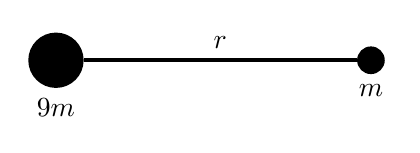
\begin{tikzpicture}
        %% masses
        \node[circle,fill,minimum size=2em] (A) at (-2,0) {};
        \node[circle,fill,minimum size=1em] (B) at (+2,0) {};
        %% Labels
        \node[anchor=north] at (A.south) {$9m$};
        \node[anchor=north] at (B.south) {$m$};
        %% Radius
        \draw[ultra thick] (A.east) -- (B.west) node[pos=0.5,anchor=south] {$r$};
    \end{tikzpicture}
    \end{center}
    Along the line shown,
        at which distance from the mass $m$ will the gravitational force on an object be least?
    \begin{multicols}{3}
    \begin{choices}
        \wrongchoice{$\dfrac{r}{2}$}
        \wrongchoice{$\dfrac{r}{3}$}
      \correctchoice{$\dfrac{r}{4}$}
        \wrongchoice{$\dfrac{r}{8}$}
        \wrongchoice{$\dfrac{r}{9}$}
    \end{choices}
    \end{multicols}
\end{question}
}

\element{ap}{
\begin{question}{gravitational-force-q21}
    A planet has a radius $R$.
    An object is dropped from a distance $2R$ from the planet's center,
        and reaches a speed of $v$ just before hitting the surface.
    The mass of the planet is:
    \begin{multicols}{3}
    \begin{choices}
        \wrongchoice{$\dfrac{Rv}{G}$}
      \correctchoice{$\dfrac{Rv^2}{2G}$}
        \wrongchoice{$\dfrac{Rv^2}{G}$}
        \wrongchoice{$\dfrac{2Rv^2}{G}$}
        \wrongchoice{$\dfrac{G}{Rv^2}$}
    \end{choices}
    \end{multicols}
\end{question}
}

\element{ap}{
\begin{question}{gravitational-force-q22}
    An object is on the surface of a planet that has twice the mass and twice the radius of the Earth.
    If the object has a mass of \SI{40}{\kilo\gram} on Earth,
        its mass on this planet will be:
    \begin{multicols}{3}
    \begin{choices}
        \wrongchoice{\SI{10}{\kilo\gram}}
        \wrongchoice{\SI{20}{\kilo\gram}}
      \correctchoice{\SI{40}{\kilo\gram}}
        \wrongchoice{\SI{80}{\kilo\gram}}
        \wrongchoice{\SI{160}{\kilo\gram}}
    \end{choices}
    \end{multicols}
\end{question}
}

\element{ap}{
\begin{question}{gravitational-force-q23}
    An object is on the surface of a planet that has half the mass and half the radius of the Earth.
    If the object weighs \SI{400}{\newton} on Earth,
        on this planet it will weigh:
    \begin{multicols}{3}
    \begin{choices}
        \wrongchoice{\SI{100}{\newton}}
        \wrongchoice{\SI{200}{\newton}}
        \wrongchoice{\SI{400}{\newton}}
      \correctchoice{\SI{800}{\newton}}
        \wrongchoice{\SI{1600}{\newton}}
    \end{choices}
    \end{multicols}
\end{question}
}

\element{ap}{
\begin{question}{gravitational-force-q24}
    An object with mass $m$ above the surface of the Earth (mass $=M$) is dropped from an altitude equal to the Earth's radius ($R$).
    At what speed will the object impact the Earth?
    \begin{multicols}{3}
    \begin{choices}
        \wrongchoice{$\sqrt{\dfrac{GM}{R}}$}
        \wrongchoice{$\sqrt{\dfrac{GM}{R^2}}$}
      \correctchoice{$\sqrt{\dfrac{2GM}{R}}$}
        \wrongchoice{$\sqrt{\dfrac{GMm}{R}}$}
        \wrongchoice{$\sqrt{\dfrac{GMm}{R^2}}$}
    \end{choices}
    \end{multicols}
\end{question}
}

\element{ap}{
\begin{question}{gravitational-force-q25}
    Two objects, each of mass $M$, are a distance $R$ apart.
    The gravitational force between them is $F$.
    If the mass of each object were tripled,
        the gravitational force between the objects would be:
    \begin{multicols}{3}
    \begin{choices}
        \wrongchoice{$\dfrac{F}{9}$}
        \wrongchoice{$\dfrac{F}{3}$}
        \wrongchoice{$3F$}
      \correctchoice{$9F$}
        \wrongchoice{$81F$}
    \end{choices}
    \end{multicols}
\end{question}
}

\element{ap}{
\begin{question}{gravitational-force-q26}
    Gravitational force $F$ exists between point objects $A$ and $B$ separated by distance $R$.
    If the mass of $A$ is doubled and distance $R$ is tripled,
        what is the new gravitational force between $A$ and $B$?
    \begin{multicols}{3}
    \begin{choices}
      \correctchoice{$\dfrac{2F}{9}$}
        \wrongchoice{$\dfrac{2F}{3}$}
        \wrongchoice{$\dfrac{3F}{2}$}
        \wrongchoice{$\dfrac{9F}{2}$}
        \wrongchoice{$6F$}
    \end{choices}
    \end{multicols}
\end{question}
}

\element{ap}{
\begin{question}{gravitational-force-q27}
    An object has a weight $W$ when it is on the surface of the Earth (radius $=R$).
    When the same object is a distance $2R$ from the center of the Earth,
        its weight will be:
    \begin{multicols}{3}
    \begin{choices}
        \wrongchoice{$4W$}
        \wrongchoice{$2W$}
        \wrongchoice{$W$}
        \wrongchoice{$\dfrac{W}{2}$}
      \correctchoice{$\dfrac{W}{4}$}
    \end{choices}
    \end{multicols}
\end{question}
}

\element{ap}{
\begin{question}{gravitational-force-q28}
    Object $A$ has mass $m$ and is on the surface of the Earth (radius $=R$).
    Object $B$ also has mass $m$,
        but is a distance $4R$ from the Earth's center.
    The ratio of the weight of $A$ to $B$ is:
    \begin{multicols}{3}
    \begin{choices}
      \correctchoice{$16:1$}
        \wrongchoice{$4:1$}
        \wrongchoice{$1:1$}
        \wrongchoice{$1:4$}
        \wrongchoice{$1:16$}
    \end{choices}
    \end{multicols}
\end{question}
}

\element{ap}{
\begin{question}{gravitational-force-q29}
    A space ship fires a weapon at a planet,
        destroying half its mass.
    The planet's inhabitants would find that
    \begin{choices}
        \wrongchoice{their mass has decreased by a factor of 2}
        \wrongchoice{their mass has been reduced by a factor 4}
      \correctchoice{their weight has been reduced by a factor of 2}
        \wrongchoice{their weight has been reduced by a factor of 4}
        \wrongchoice{their mass and weight are both reduced by a factor of 2}
    \end{choices}
\end{question}
}

\element{ap}{
\begin{question}{gravitational-force-q30}
    If the distance between the center of gravity of a satellite and the center of gravity of the Earth is halved and the mass of the satellite is doubled,
        then:
    \begin{choices}
        \wrongchoice{the force of gravity is halved}
        \wrongchoice{the force of gravity is doubled}
        \wrongchoice{the force of gravity is unchanged}
        \wrongchoice{the force of gravity is quadrupled}
      \correctchoice{the force of gravity is increased by a factor of 8}
    \end{choices}
\end{question}
}

\element{ap}{
\begin{question}{gravitational-force-q31}
    A person with a mass of \SI{75}{\kilo\gram} goes to a planet with twice the radius and half the mass of earth.
    What is their weight on this planet?
    \begin{multicols}{2}
    \begin{choices}
        \wrongchoice{\SI{87.5}{\newton}}
      \correctchoice{\SI{93.75}{\newton}}
        \wrongchoice{\SI{187.5}{\newton}}
        \wrongchoice{\SI{250.25}{\newton}}
        \wrongchoice{\SI{1500}{\newton}}
    \end{choices}
    \end{multicols}
\end{question}
}

\element{ap}{
\begin{question}{gravitational-force-q32}
    A person with a mass of \SI{75}{\kilo\gram} goes to a planet with twice the radius and half the mass of earth.
    What is their mass on this planet?
    \begin{multicols}{3}
    \begin{choices}
      \correctchoice{\SI{75}{\kilo\gram}}
        \wrongchoice{\SI{94}{\kilo\gram}}
        \wrongchoice{\SI{150}{\kilo\gram}}
        \wrongchoice{\SI{300}{\kilo\gram}}
        \wrongchoice{\SI{350}{\kilo\gram}}
    \end{choices}
    \end{multicols}
\end{question}
}


\endinput


